%!TEX root = main.tex
\section{Introduction}


%Exploring multidiemnsional dataset is hard
\par Visual data exploration is the {\em de facto} first step in understanding multi-dimensional datasets. This exploration enables analysts to identify trends and patterns, generate and verify hypotheses, and detect outliers and anomalies. However, as datasets grow in size and complexity, visual data exploration becomes challenging. In particular, to
\change{understand how a global pattern came about,
an analyst may need to explore different subsets of the data
to see whether the same or different pattern manifests itself
in these subsets.}
\change{Unfortunately, manually}
generating and examining each visualization
in this space of data subsets
(which grows exponentially in \change{the} number of attributes)
presents a major bottleneck \change{during exploration}.
%Drill-Down for exploration
\begin{figure}[ht!]
% 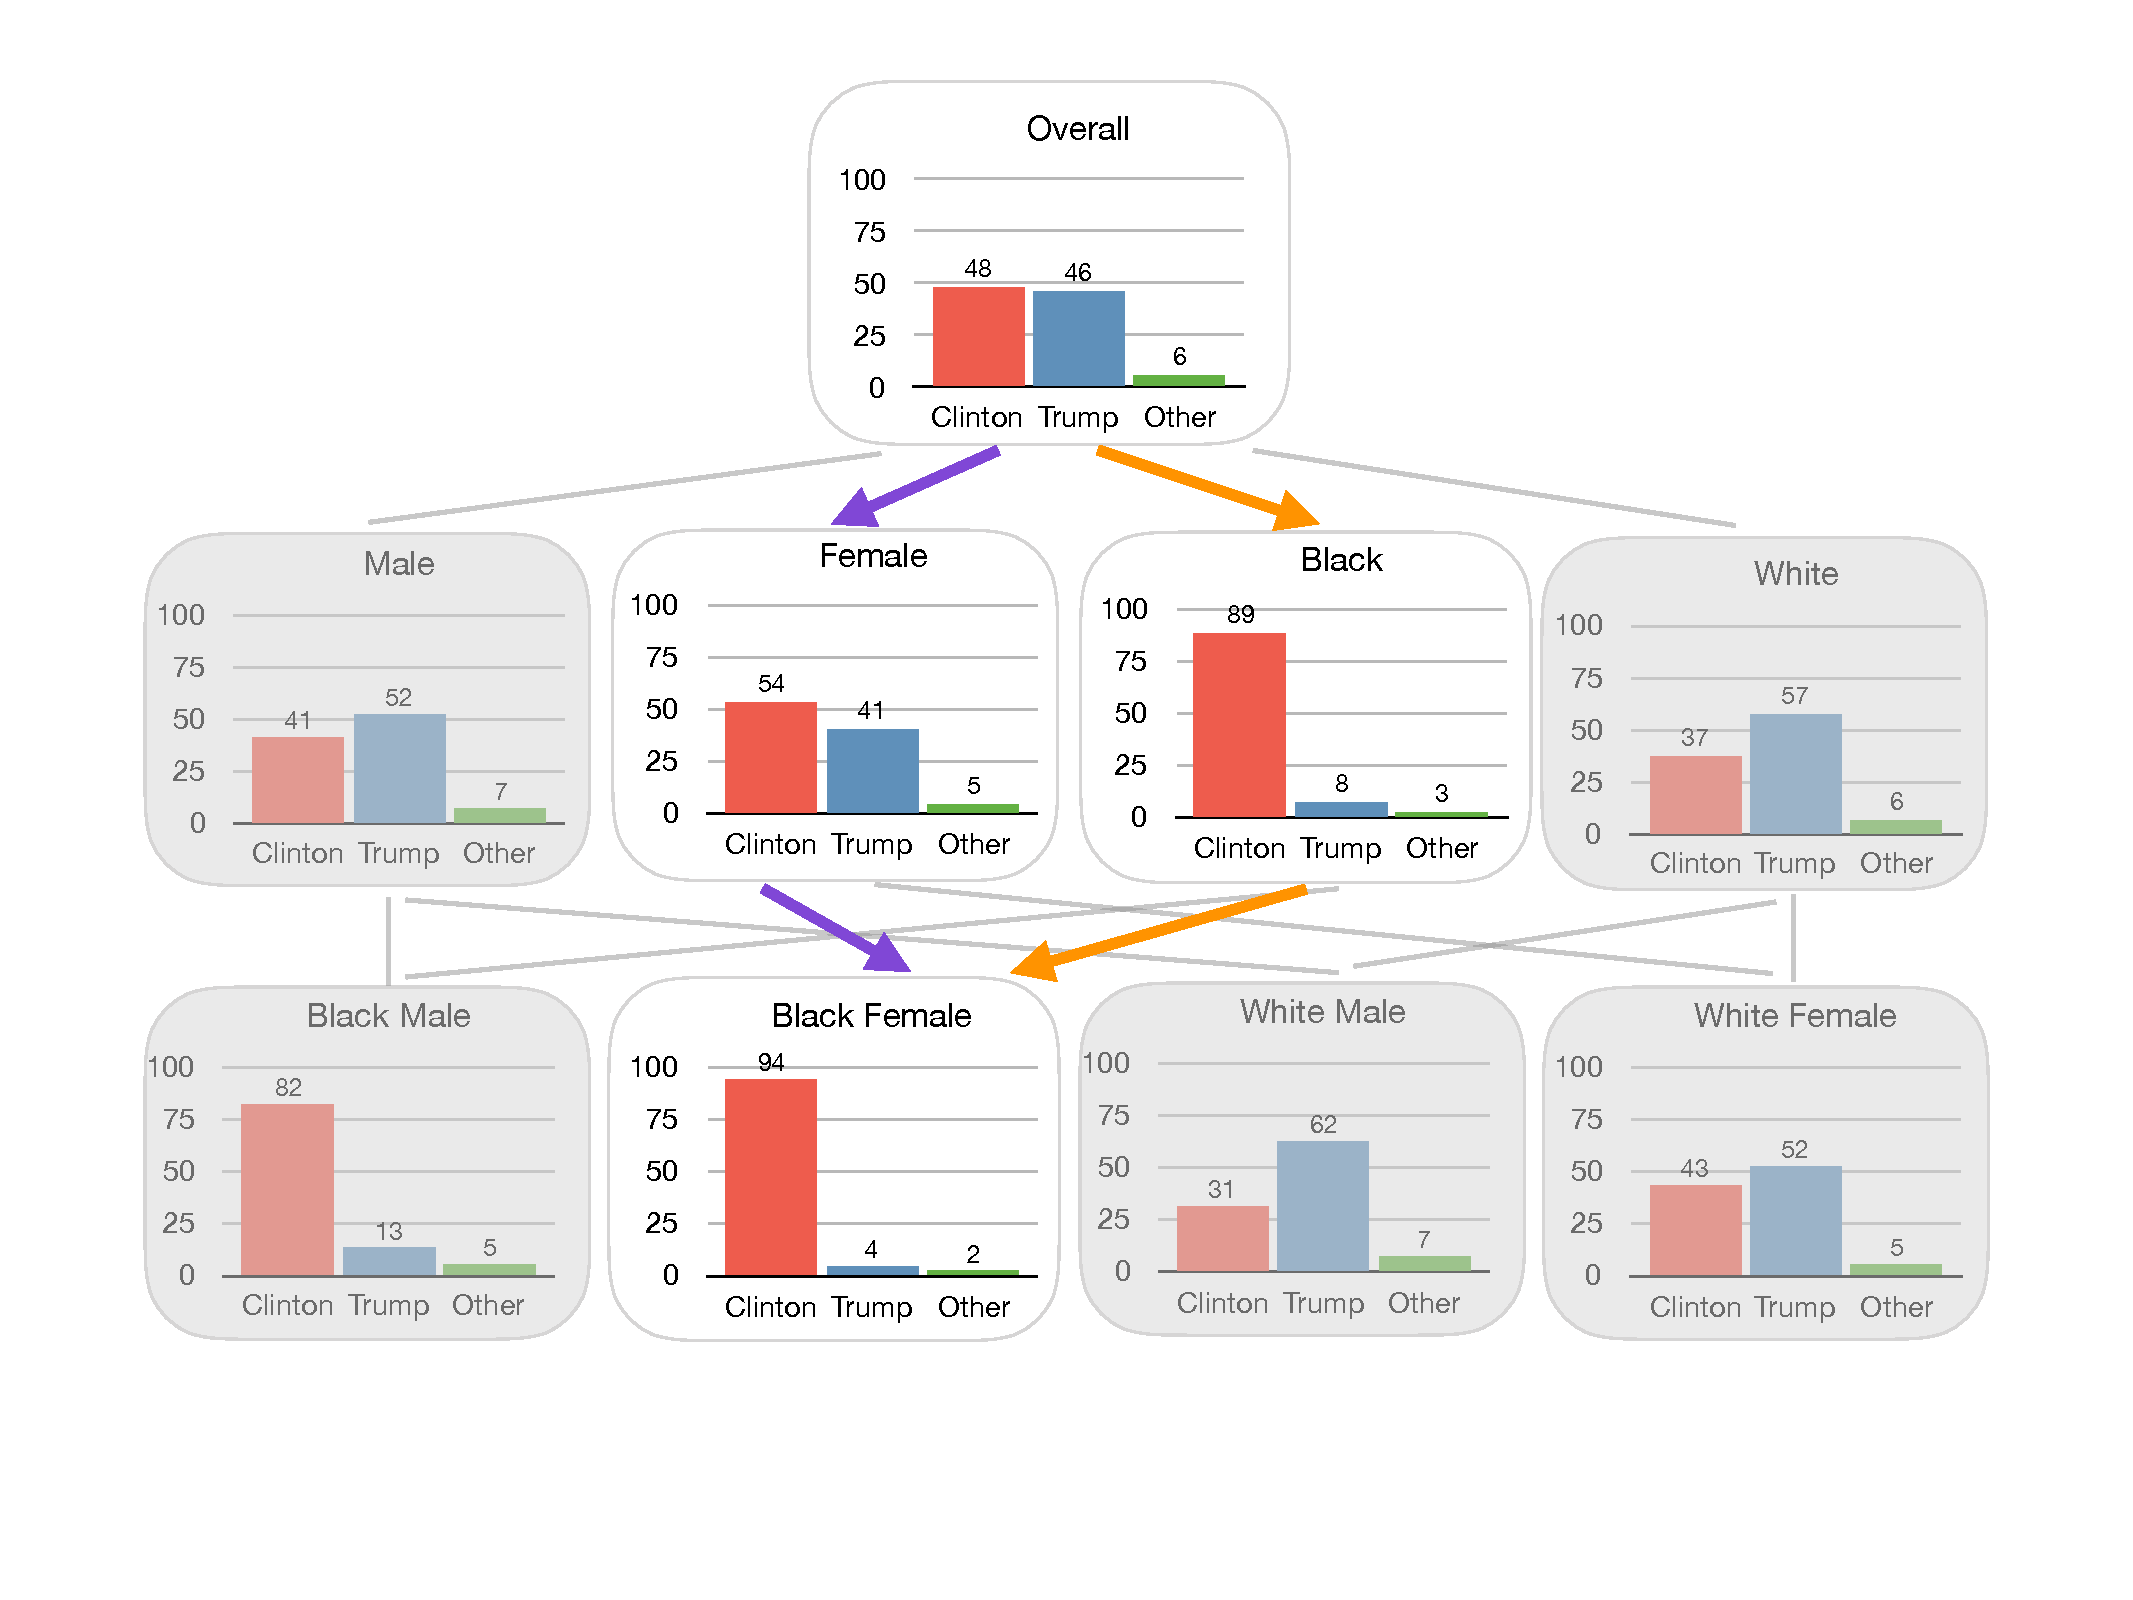
\includegraphics[width=\linewidth]{figures/elections_example_lattice.pdf}
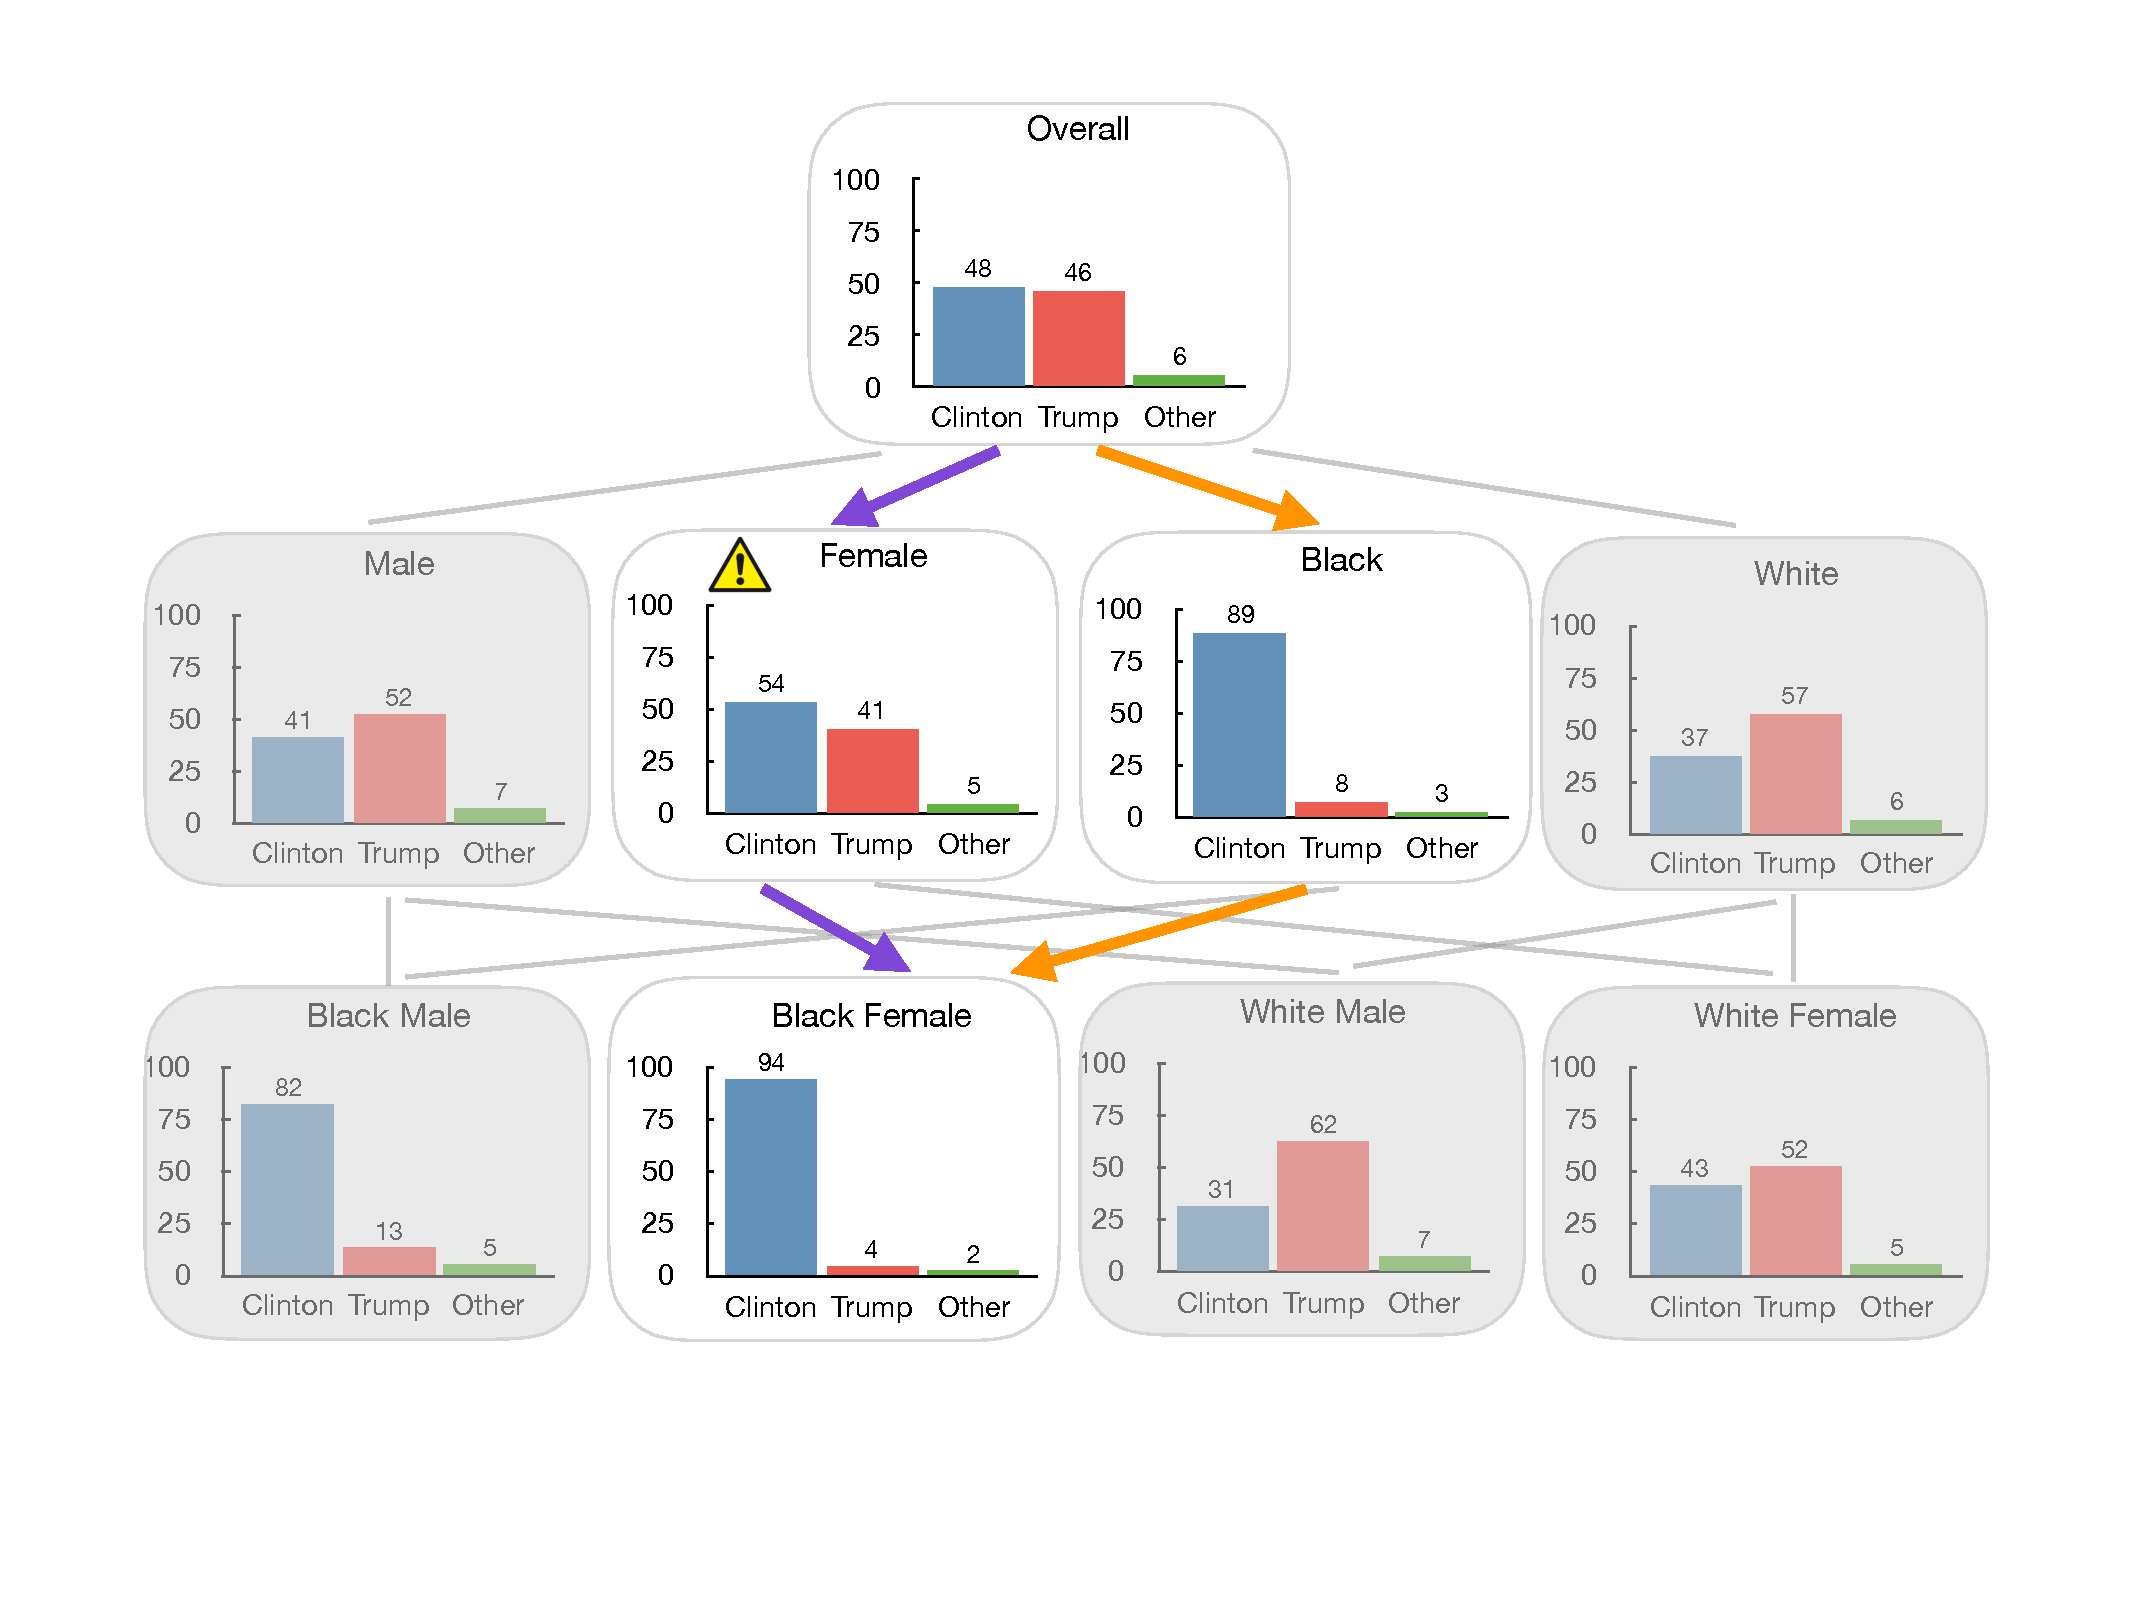
\includegraphics[width=0.95\linewidth]{figures/elections_example_lattice_teaser.pdf}
\vspace{-5pt}
\caption{Example data subset lattice from the 2016 US election dataset illustrating the drill-down fallacy along the purple path as opposed to the informative orange path.}
\label{fig:elections_example}
\vspace{-10pt}
\end{figure}
\par One way of navigating this combinatorial space
is to perform \change{{\em drill-downs}}
on the space\change{---a {\em lattice}---}of data subsets.
For example, a campaign manager
who is interested in understanding
voting patterns across different
demographics (say, race, gender, or social class)
using the 2016 US election exit polls~\cite{exitpolls}
may first generate a bar chart for the entire population,
where the x-axis shows the election candidates
and the y-axis \change{shows} the percentage of votes for each of these candidates.
In Figure~\ref{fig:elections_example},
the visualization at the top of the lattice
corresponds to the overall population.
The analyst may then \change{use their intuition to}
drill down to specific demographics of interest,
say gender-based demographics,
by generating bar charts for female voters \change{by following the purple path},
as shown in the second visualization
at the second row of Figure~\ref{fig:elections_example}\change{,
and then to the visualization corresponding to \blkfem voters
in the third row}.
%Challenges associated with drill-down

\stitle{\change{Challenges with Manual Drill-down.}}
There are three challenges \change{associated
with manual drill downs:}

\smallskip
\noindent
First, it is often not clear which attributes to
drill-down on. Analysts may use their
intuition \change{to select} the drill-down attribute,
but such arbitrary exploration  may lead to
large portions of the lattice being \change{{\em unexplored}---leading
to missed insights}.

\smallskip
\noindent
Second, \change{a path taken by analysts in an uninformed
manner may lead to visualizations
that are {\em not very surprising or insightful}}.
For example, an analyst may end up
wasting effort by drilling down
from the \blk visualization to the \blkfem one in Figure~\ref{fig:elections_example},
since the two distributions are similar and therefore not very surprising.

\smallskip
\noindent
Third, an analyst \change{may encounter a
{\bf {\em drill-down fallacy}}---a new class of errors
in reasoning we identify---where incomplete insights result from potentially confounding factors not explored along a drill-down path}. As shown in Figure~\ref{fig:elections_example}, an analyst can arrive at the \blkfem visualization \change{via} the purple or the orange drill-down path. An analyst who followed the purple path
may be surprised at how drastically the \blkfem
voting behavior differs from that of \fem.
However, this behavior is not surprising if
the analyst had gone down the orange path that we saw earlier, where the proper reference (i.e., the distribution for \blk)
explains the vote distribution for \blkfem.
In other words, even though the vote distribution for \blkfem is very different from that of \fem,
the phenomenon can be explained by a more general ``root cause'' attributed to the voting behavior for the \blk
community \change{as a whole}.
\change{Attributing an overly specific cause to an effect,
while ignoring the actual, more general cause,
}not only leads to less interpretable explanations for the observed visualizations, but can also \change{lead to erroneous} decision-making. For example, for the campaign manager, this could lead to \change{incorrect} allocation of campaign funds. \change{To prevent analysts from falling prey to such drill-down fallacies---consisting of misleadingly ``surprising''
local deviations in trend during drill-down
(\fem $\rightarrow$ \blkfem)---it is important to preserve the proper parent reference (\blk)
to contextualize the behavior of the visualization of interest (\blkfem).} One approach to avoid this fallacy
is to \change{exhaustively} explore all potential drill-down paths. Unfortunately, this approach does not
scale.

\par \change{While there have been a number of statistical
reasoning fallacies that have been identified
in visual analytics, including Simpson's paradox~\cite{Guo2017,Armstrong2014}, multiple comparisons~\cite{Zgraggen2018CHI}, and selection bias~\cite{Gotz2016},
to the best of our knowledge,
our paper is the first to identify the drill-down fallacy,
a common fallacy that appears during manual
data exploration.
There have been efforts
to develop visualization recommendation
systems~\cite{Lee2018,Vartak2015} that
assist or accelerate the process of visual
data exploration~\cite{Vartak2015,Siddiqui2017,Wongsuphasawat2016,Kandel2012,Joglekar2015,Binnig2017,Key2012},
none of these systems have provided
a conclusive solution to the problem of aiding drill-downs
to explore data subsets,
while avoiding drill-down fallacies.
We discuss
related work in detail in Section~\ref{sec:related}.}

 \par
 \stitle{\change{\system with Safety, Saliency, and Succinctness.}}
We present a visual data exploration tool, titled \system,
 that addresses the three aforementioned
 challenges of exploration \change{by espousing}
 three principles:
 (i) \textbf{Safety}
 (i.e., ensure that proper
 references are present to
 avoid drill-down fallacies),
 (ii) \textbf{Saliency}
 (i.e., identify interesting visualizations
 that convey new information or insights),
 and (iii) \change{\textbf{Succinctness}}
 (i.e., \change{convey only the key
 insights in the} dataset).
 To facilitate safety, we develop a
 notion of \emph{informativeness}---the capability
 of a reference \change{parent}
 visualization to explain the visualization of interest.
 To facilitate saliency,
 we characterize the notion of \emph{interestingness}---the
 difference between a visualization and
 its informative reference
 in terms of underlying data distribution.
 Finally, to facilitate \change{succinctness,
 we embrace a collective measure of
 visualization utility by recommending a {\em compact}
 connected network of visualizations}.
 Based on these three principles,
 \change{\system\ {\em  automatically identifies a
 {\bf \em compact} network of  {\bf \em informative} and  {\bf \em interesting} visualizations
 that collectively convey the key
 insights in a dataset}. Our user study results demonstrate that
 \system can help analysts gain a better understanding
 of the dataset and help them accomplish a variety of tasks}.
 Our contributions include:
\begin{denselist}
\item Identifying
the notion of \change{a {\em drill-down fallacy}};
\item Introducing the concept of \emph{informativeness}
that helps identify insights
that arise from something
\change{that holds
in the data (as opposed to confounding local phenomena)};
\item \change{Extending the concept of informativeness to a
measure to quantify the benefit of a network of visualizations};
\item Designing \system, \change{which efficiently and automatically identifies} a network of visualizations \change{conveying} the key insights in a dataset; and
%that builds a dashboard by
\item Demonstrating the efficacy of \change{\system} through a user study evaluation on how well users can retrieve interesting visualizations, judge the importance of attributes, and predict unseen visualizations, against two baselines.
\end{denselist}
